\documentclass[main.tex]{subfiles}
\begin{document}

\section{Analog results}
Over 4 hours of measurements $17.3\cdot 10^{6}$ events were recorded by the analog setup. The immediate output is 4 tdc spectrums Giving the time differences for NE213 hits and the respective YAPs. qdc spectra, one for each yap, and two qdc spectra for the NE213 detector (one longgate and one shortgate). 

\subsection{YAP QDC spectrum}
Write about scattered gammas that are both stop and start signals. Geometry dependent. Analog setup only records when there is a ToF coincidence, so scattered gammas end up dominating the yap qdc spectrum, which leads to the yap closest to the NE213 always having the largest gamma peak in the ToF spectrum. The Digital setup records everything passing the threshold, so by comparing with it we get an idea of the real gamma distrubution.

\newpage
\subsection{NE213 QDC spectrum}
The energy registered in the longgate QDC is shown in fig \ref{fig:qdc_a}. 'A peak is clearly visible at around 4.4 $MeV_{ec}$. This is the energy of the gammas emmited by the deexciting $^{12}C$ atoms. ---Write about other peak---

\subsection{ToF spectrum}
-ToF spectrum

\begin{figure}[ht]
    \centering
        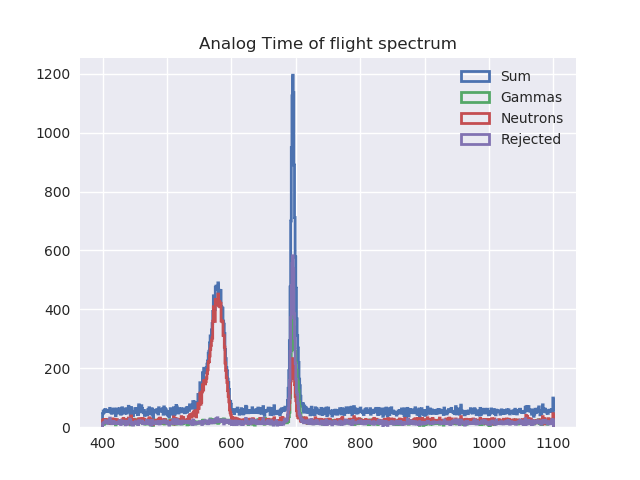
\includegraphics[scale=.75]{AnalogResults/tof_psd.png}
        \caption{The time of flight spectrum.}
    \label{fig:A_TOF}
\end{figure}
\begin{figure}[ht]
    \centering
        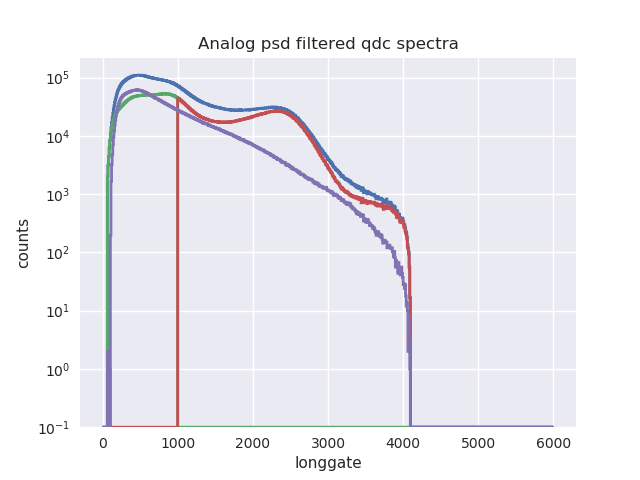
\includegraphics[scale=.75]{AnalogResults/qdc_psd.png}
        \caption{Analog QDC spectrum.}
    \label{fig:qdc_a}
\end{figure}


\subsection{Pulse shape discrimination}
\subsubsection{Charge comparison method}
Since neutrons and gammas interact differently in the NE213 detector their signal has different shape and duration. This makes it possible to discriminate between neutrons and gammas.



\begin{figure}
    \centering
    \begin{subfigure}[b]{0.9\textwidth}
        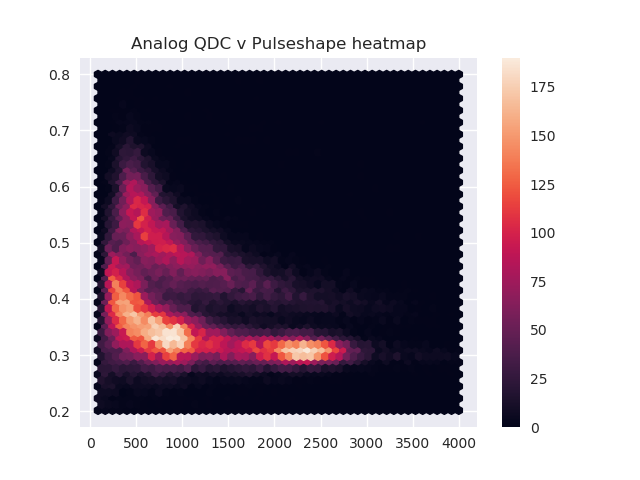
\includegraphics[width=\textwidth]{AnalogResults/psd_hexbin.png}
        \caption{Hexbin heatmap of Pulse shape distribution. The upper band is neutrons and the lower one is gammas.}
        \label{fig:hex_a}
    \end{subfigure}
    \begin{subfigure}[b]{0.9\textwidth}
        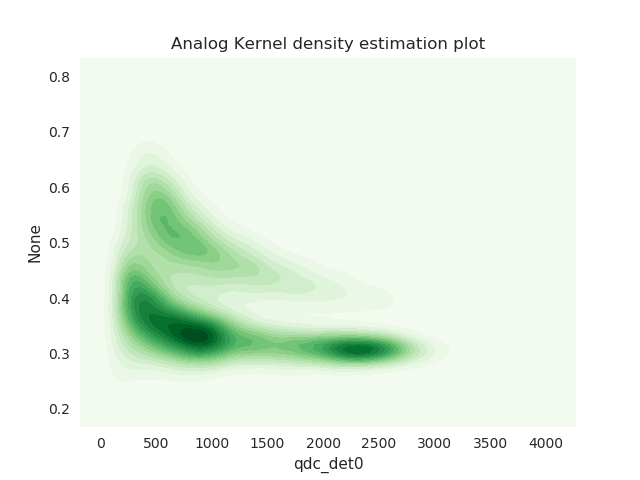
\includegraphics[width=\textwidth]{AnalogResults/psd_kde.png}
        \caption{Kernel density estimation plot of the pulse shape spectrum. The upper band is neutrons and the lower one is gammas.}
        \label{fig:kde_a}
    \end{subfigure}
\label{fig:animals}
\end{figure}

\subsection{Pulse shape v ToF}
\begin{figure}[ht]
    \centering
        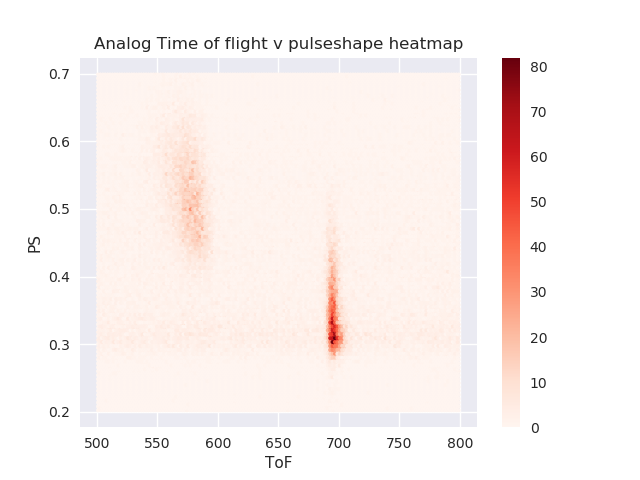
\includegraphics[scale=.85]{AnalogResults/ps_tof.png}
        \caption{heatmap of ToF vs pulse shape.}
    \label{fig:tof_ps_a} 
\end{figure}

\newpage
\subsection{PSD filtered QDC spectra}
\begin{figure}[ht]
    \centering
        \includegraphics[scale=.75]{AnalogResults/qdc_filtered_psd.png}
        \caption{The digital QDC spectrum.}
    \label{fig:D_QDC}
\end{figure}

\newpage
\subsection{PSD filtered Time of flight spectrum}
\begin{figure}[ht!]
    \centering
        \includegraphics[scale=.75]{AnalogResults/tof_filtered_psd.png}
        \caption{The digital time of flight spectrum, filtered using psd classification.}
    \label{fig:D_PSD_TOF} 
\end{figure}


\end{document}